

\begin{frame}{Repère orthogonal 2D}
    \small
    Un repère orthogonal 2D est une croix orientée par un angle $\theta$.
    \newline
    \newline
    \begin{minipage}{0.46\textwidth}
        \centering
        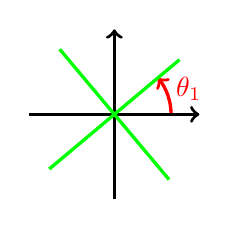
\begin{tikzpicture}[very thick, scale=.9]
            \draw[->, red] (.8, 0) arc (0:40:.8) node[right,pos=.66] {$\theta_1$};
            \draw[->] (180:1.2) -- (0:1.2);
            \draw[->] (-90:1.2) -- (90:1.2);
            \draw[green] (220:1.2) -- (40:1.2);
            \draw[green] (310:1.2) -- (130:1.2);
        \end{tikzpicture}
    \end{minipage}
    \hfill
    \begin{minipage}{0.46\textwidth}
        \centering
        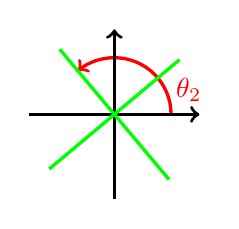
\begin{tikzpicture}[very thick, scale=.9]
            \draw[->, red] (.8, 0) arc (0:130:.8) node[right,pos=.2] {$\theta_2$};
            \draw[->] (180:1.2) -- (0:1.2);
            \draw[->] (-90:1.2) -- (90:1.2);
            \draw[green] (220:1.2) -- (40:1.2);
            \draw[green] (310:1.2) -- (130:1.2);
        \end{tikzpicture}
    \end{minipage}
    
    \vfill
    
    \small
    Une croix étant $\pi/2$-périodique, nous la représentons par $(X, Y) = (\cos4\theta, \sin4\theta)$ pour éviter les problèmes de périodicité.
    \newline
    \newline
    \begin{minipage}{0.4\textwidth}
        \centering
        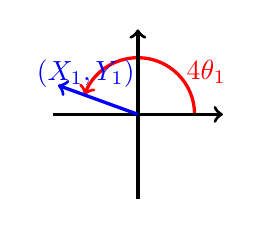
\begin{tikzpicture}[very thick, scale=.9]
            \draw[->, red] (.8, 0) arc (0:160:.8) node[right,pos=.3] {$4\theta_1$};
            \draw[->] (180:1.2) -- (0:1.2);
            \draw[->] (-90:1.2) -- (90:1.2);
            \draw[->, blue] (340:0) -- (160:1.2) node[right,pos=1.4] {$(X_1, Y_1)$};
        \end{tikzpicture}
    \end{minipage}
    \hfill
    \begin{minipage}{0.53\textwidth}
        \centering
        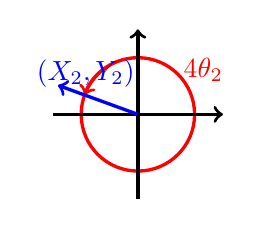
\begin{tikzpicture}[very thick, scale=.9]
            \draw[->, red] (.8, 0) arc (0:520:.8) node[right,pos=.1] {$4\theta_2$};
            \draw[->] (180:1.2) -- (0:1.2);
            \draw[->] (-90:1.2) -- (90:1.2);
            \draw[->, blue] (340:0) -- (160:1.2) node[right,pos=1.4] {$(X_2, Y_2)$};
        \end{tikzpicture}
    \end{minipage}
\end{frame}

\begin{frame}{Champ de repère 2D plat}
    \small
    Pour optimiser un champ de repère 2D plat sans problème de périodicité, nous optimisons 
    les vecteurs de représentations $(X, Y)$:
    \small{
    \begin{equation*}
    \begin{array}{ll}
    \underset{X, Y}{\argmin} & \underset{t \in T}{\displaystyle\sum} \underset{t' \in \mathcal{N}(t)}{\displaystyle\sum} \left|\left|\ \begin{pmatrix} X_{t'}\\ Y_{t'}\end{pmatrix} - \begin{pmatrix} X_{t}\\ Y_{t}\end{pmatrix} \right|\right|^2, \\
    \text{sous contrainte: } & \forall t \in T_b, \begin{pmatrix} X_{t}\\ Y_{t}\end{pmatrix} = \begin{pmatrix} \cos4\eta_t\\ \sin4\eta_t\end{pmatrix}.
    \end{array}
    \end{equation*}
    }
    Puis nous retrouvons les angles $\theta$ du champ de repère:
    $$ \forall t \in T,\ \  \theta_t = \frac{1}{4}\tan^{-1}\frac{Y_t}{X_t}$$

\end{frame}


\begin{frame}{Problèmes des bords à petits angles}

    \begin{center}
    \begin{tabular}{c|c|c|c|c}
    % First row: angle text
    $\alpha_v=10^{\circ}$ & $\alpha_v=90^{\circ}$ & $\alpha_v=180^{\circ}$ & $\alpha_v=270^{\circ}$ & $\alpha_v=350^{\circ}$ \\
    \hline
    % Second row: TikZ diagrams
    \begin{minipage}{0.14\textwidth}
    \centering
    \begin{tikzpicture}[scale=0.2]
    % Lines forming a 10° angle
    \draw (0,0) -- (0,3);
    \draw (0,0) -- ({3*sin(10)},{3*cos(10)});
    \node[rotate=40, green, scale=2] at (0.2,2) {$\times$}; % Added cross
    \end{tikzpicture}
    \end{minipage}
    &
    \begin{minipage}{0.14\textwidth}
    \centering
    \begin{tikzpicture}[scale=0.2]
    \only<2-2> {
    \draw[red] (0.0,0.0) rectangle (3.0,3.0); % Added quadrilateral
    }
    % Lines forming a 90° angle
    \draw (0,0) -- (0,3);
    \draw (0,0) -- (3,0);
    \node[rotate=45, green, scale=2] at (1.5,1.5) {$\times$}; % Added cross
    \end{tikzpicture}
    \end{minipage}
    &
    \begin{minipage}{0.17\textwidth}
    \centering
    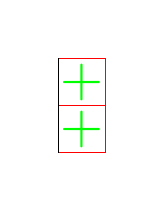
\begin{tikzpicture}[scale=0.2]
    \only<2-2> {
    \draw[red] (0.0,0.0) rectangle (3.0,3.0); % Added quadrilateral
     \draw[red] (0.0,-3.0) rectangle (3.0,0.0); % Added quadrilateral
    }
    % Lines forming a 180° angle
    \draw (0,0) -- (0,3);
    \draw (0,0) -- (0,-3);
    \node[rotate=45, green, scale=2] at (1.5,1.5) {$\times$}; % Added cross
    \node[rotate=45, green, scale=2] at (1.5,-1.5) {$\times$}; % Added cross
    \end{tikzpicture}
    \end{minipage}
    &
    \begin{minipage}{0.17\textwidth}
    \centering
    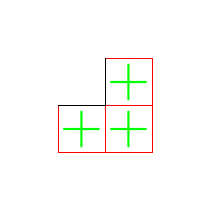
\begin{tikzpicture}[scale=0.2]
    % Lines forming a 270° angle
    \only<2-2> {
     \draw[red] (0.0,0.0) rectangle (3.0,3.0); % Added quadrilateral
     \draw[red] (0.0,-3.0) rectangle (3.0,0.0); % Added quadrilateral
     \draw[red] (-3.0,-3.0) rectangle (0.0,0.0); % Added quadrilateral
    }
    \draw (0,0) -- (0,3);
    \draw (0,0) -- (-3,0);
    \node[rotate=45, green, scale=2] at (1.5,1.5) {$\times$}; % Added cross
    \node[rotate=45, green, scale=2] at (1.5,-1.5) {$\times$}; % Added cross
    \node[rotate=45, green, scale=2] at (-1.5,-1.5) {$\times$}; % Added cross
    \end{tikzpicture}
    \end{minipage}
    &
    \begin{minipage}{0.17\textwidth}
    \centering
    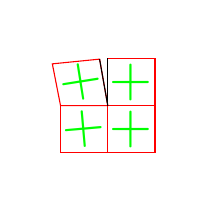
\begin{tikzpicture}[scale=0.2]
    % Lines forming a 350° angle
    \only<2-2> {
     \draw[red] (0.0,0.0) rectangle (3.0,3.0); % Added quadrilateral
     \draw[red] (0.0,-3.0) rectangle (3.0,0.0); % Added quadrilateral
     \draw[red] (-3.0,-3.0) rectangle (0.0,0.0); % Added quadrilateral
     \draw[red] (-3.0,0.0) -- (0.0,0.0) -- ({3*sin(350)},{3*cos(350)}) -- ({3*sin(350)-3},{3*cos(350) - 0.3}) -- cycle; % Added parallelogram
    }
    \draw (0,0) -- (0,3);
    \draw (0,0) -- ({3*sin(350)},{3*cos(350)});
    \node[rotate=45, green, scale=2] at (1.5,1.5) {$\times$}; % Added cross
    \node[rotate=45, green, scale=2] at (1.5,-1.5) {$\times$}; % Added cross
    \node[rotate=50, green, scale=2] at (-1.5,-1.5) {$\times$}; % Added cross
    \node[rotate=54, green, scale=2] at (-1.7,1.5) {$\times$}; % Added cross
    \end{tikzpicture}
    \end{minipage}
    \end{tabular}
    
    \only<2-2>{
        \vspace{0.3cm}
        Un champ de repère orthogonal produit un maillage quadrilatère de valence de bord: $$k_v = \text{arrondi} \left( \frac{\alpha_v}{90} \right)$$
    
        Problème: pour $\alpha_v < 45^\circ$, on obtient une valence $k_v = 0$ qui fait échouer la méthode. %le sommet de bord est donné de valence 0, ce qui fait échouer la méthode.
    }
    \end{center}
    
\end{frame}

\begin{frame}{Problèmes avec les modèles CAO}
    \begin{center}
        \includegraphics[width=0.99\linewidth]{img/cadff/teaser2}
    \end{center}
\end{frame}
    
\begin{frame}{Intuition de la contribution}
    \begin{center}
        \includegraphics[width=0.9\linewidth]{img/new_images/flat_tri_annot.png}
        \includegraphics[width=0.9\linewidth]{img/new_images/surface_tri_annot.png}
        \small{
            \textit{Modifier la définition du transport parallèle permet de transformer les petits angles en angles de 90°.}
        }
    \end{center}
\end{frame}
\begin{frame}{Modification de la définition du transport parallèle pour empêcher les petits angles}

    \begin{center}
    \begin{tikzpicture}[scale=1]
    % Triangle 1
    \fill[blue!20] (0,0) -- (8,0) -- (8,1) -- cycle;
    
    % Triangle 2
    \fill[red!20] (0,0) -- (8,0) -- (8,-1) -- cycle;
    
    \node at ($ (2,0) $) {$\alpha_v = 14^{\circ}$}; % Shifted to the right
    \draw[->, blue] ($ (6,0) + (0,-0.2) $) to [bend right=45] ($ (6,0) + (0,0.2) $); % Flèche going from bottom to top
    \node[blue] at ($ (6,0) + (1,0) $) {$\gamma = 0^{\circ}$};

    \end{tikzpicture}

    \vspace{.5cm} % Adjust this value to increase or decrease the space

    \begin{tikzpicture}[scale=1]
    % Triangle 1
    \fill[blue!20] (0,0) -- (8,0) -- (8,1) -- cycle;
    
    % Triangle 2
    \fill[red!20] (0,0) -- (8,0) -- (8,-1) -- cycle;
    
    \node at ($ (2,0) $) {$\alpha_v + K_v = 90^{\circ}$}; % Shifted to the right
    \draw[->, blue] ($ (6,0) + (0,-0.2) $) to [bend right=45] ($ (6,0) + (0,0.2) $); % Flèche going from bottom to top
    \node[blue] at ($ (6,0) + (1,0) $) {$\gamma = 76^{\circ}$};

    \end{tikzpicture}
    \end{center}
    
\end{frame}

\begin{frame}{Diffusion of $\gamma$}

    \begin{minipage}{0.59\textwidth}
    \begin{figure}
      \centering
      \only<1>{\includegraphics[width=0.79\linewidth]{img/cadff/sharp0}
      \caption{Champ le plus lisse}}
      \includegraphics[width=0.79\linewidth]{img/cadff/sharp1}
      \caption{Singularité sur le 1-voisinage}
      \only<2>{\includegraphics[width=0.79\linewidth]{img/cadff/sharp2}
      \caption{Propagation globale de la courbure}}
    \end{figure}
    \end{minipage}%
    \begin{minipage}{0.39\textwidth}
        Pour tous les sommets de coin à petit angle \(v\):\\
        On fixe \(K_v = 90 - \theta_v\).
        \only<2>{Puis: \(\argmin \displaystyle\sum_{tt'}|\gamma_{tt'}|^2\)}
        
        \vspace{1em}
        \begin{block}{Contraintes:}
            \begin{itemize}
                \item \(\displaystyle\sum_{v \in \mathcal{V}} K_v =0\) 
                \item $ \forall v,\displaystyle\sum_{tt' \in \mathcal{N}(v)}\gamma_{tt'} = K_v$
            \end{itemize}
        \end{block}
    \end{minipage}
    
\end{frame}

\begin{frame}{Optimisation d'un champ adapté aux modèles CAO}

    Pour chaque paire de triangles adjacents $(t, t')$, on calcule la matrice de rotation 
    induite par $\gamma_{tt'}$:
    $$R_{tt'} = \begin{pmatrix}\cos4\gamma_{tt'} & -\sin4\gamma_{tt'} \\ \sin4\gamma_{tt'} & \cos4\gamma_{tt'} \end{pmatrix}$$
    Le problème d'optimisation devient alors :
   
    \begin{equation*}
        \begin{array}{ll}
        \underset{X, Y}{\argmin} & \underset{t \in T}{\displaystyle\sum} \underset{t' \in \mathcal{N}(t)}{\displaystyle\sum} \left|\left|\ \begin{pmatrix} X_{t'}\\ Y_{t'}\end{pmatrix} - R_{tt'} \begin{pmatrix} X_{t}\\ Y_{t}\end{pmatrix} \right|\right|^2, \\
        \text{sous contrainte: } & \forall t \in T_b, \begin{pmatrix} X_{t}\\ Y_{t}\end{pmatrix} = \begin{pmatrix} \cos4\eta_t\\ \sin4\eta_t\end{pmatrix}.
        \end{array}
        \label{eq:cadff_ff_2D_surface_optim}
    \end{equation*}
    
\end{frame}